\documentclass[t]{beamer}
\usetheme{Copenhagen}
\setbeamertemplate{headline}{} % remove toc from headers
\beamertemplatenavigationsymbolsempty

\usepackage{amsmath, array, tikz, bm, pgfplots, tcolorbox, graphicx, venndiagram, color, colortbl, xfrac}
\pgfplotsset{compat = 1.16}
\usepgfplotslibrary{statistics}
\usetikzlibrary{calc}

\title{Confidence Intervals}
\author{}
\date{}

\AtBeginSection[]
{
  \begin{frame}
    \frametitle{Objectives}
    \tableofcontents[currentsection]
  \end{frame}
}

\begin{document}

\pgfmathdeclarefunction{gauss}{2}{%
  \pgfmathparse{1/(#2*sqrt(2*pi))*exp(-((x-#1)^2)/(2*#2^2))}%
}

\begin{frame} 
\maketitle
\end{frame}

\section{Determine confidence intervals for population mean}

\begin{frame}{How Close Are We to the Population Mean?}
In the last section, we looked at sampling distributions of the sample mean (and proportion too). Throughout the series, we've used computer simulations to examine statistical concepts. \newline\\	\pause

However, in real life, there are factors that can limit the number of studies and samples we can take: time, cost, etc. \newline\\	\pause

So, for our samples, how confident are we that they contain the population mean?	\newline\\	\pause

That is where confidence intervals come into play.
\end{frame}

\begin{frame}{How Confident Are We?}
\begin{tcolorbox}[colframe=green!20!black, colback = green!30!white,title=\textbf{Confidence Interval}]
A \textbf{confidence interval} for a population parameter is an estimate of possible values for the parameter with a \emph{given} certain level of confidence.
\end{tcolorbox}
\bigskip \pause

\begin{tcolorbox}[colframe=green!20!black, colback = green!30!white,title=\textbf{Confidence Level}]
The \textbf{confidence level}, or \textbf{level of confidence}, is the percentage of the number of times our confidence intervals will contain the population parameter.
\end{tcolorbox}
\bigskip \pause

Typical confidence levels are 90\%, 95\%, 98\%, and 99\%.
\end{frame}

\begin{frame}{Confidence Interval Setup}
A confidence interval for a population parameter is in the form
\[\text{point estimate} \pm \text{margin of error}\]	\pause

\begin{tcolorbox}[colframe=green!20!black, colback = green!30!white,title=\textbf{Point Estimate}]
A \textbf{point estimate} is a value based on our sample data that represents a reasonable value of the population parameter.
\end{tcolorbox}
\bigskip \pause

The margin of error is in the form
\begin{center}
critical value $\times$ standard error
\end{center}
\end{frame}

\begin{frame}{Critical Values}
Critical values are typically in the form $z_{\alpha/2}$ where	
\begin{center}
\begin{tikzpicture}[scale=0.8]
\begin{axis}[
axis lines = left, xmin = -3.5, xmax = 3.5, ymin = 0, ymax = 0.45, xticklabels = {},
xtick style={draw=none}, xlabel = {z Score}, ylabel = {Probability}
]
\addplot [draw = none, fill = green, domain = -3.5:-1.5] {gauss(0,1)} \closedcycle;
\addplot [draw = none, fill = green, domain = 1.5:3.5] {gauss(0,1)} \closedcycle;
\addplot [color=blue, samples=200,thick, domain=-3.5:3.5] {gauss(0,1)};
\draw [<->,>=stealth,thick] (axis cs: -1.5,0.05) -- (axis cs: 1.5,0.05) node [above, midway] {$\bm{1-\alpha}$};
\draw [->,>=stealth,thick] (axis cs: -2.65,0.1) node [above] {$\bm{\alpha/2}$} -- (axis cs: -2.05,0.015);
\draw [->,>=stealth,thick] (axis cs: 2.65,0.1) node [above] {$\bm{\alpha/2}$} -- (axis cs: 2.05,0.015);
\end{axis}
\end{tikzpicture}
\end{center}
\end{frame}

\begin{frame}{Common Critical Values of $z_{\alpha/2}$}
\begin{center}
\begin{tabular}{c|c}
Confidence Level & Critical Value of $z_{\alpha/2}$ \\ \hline
\onslide<2->{90\%} & \onslide<2->{$\pm 1.645$} \\[8pt]
\onslide<3->{95\%} & \onslide<3->{$\pm 1.96$} \\[8pt]
\onslide<4->{98\%} & \onslide<4->{$\pm 2.326$} \\[8pt]
\onslide<5->{99\%} & \onslide<5->{$\pm 2.576$} \\[8pt]
\end{tabular}
\end{center}
\onslide<6->{Notice the higher the confidence level, the further away from $z = 0$ the critical value is.}	\newline\\
\onslide<7->{The standard error is still $\frac{\sigma}{\sqrt{n}}$}	\newline\\
\onslide<8->{\emph{Note:} If $\sigma$ is unknown, you can use the sample standard deviation, $s$, when the sample size is large enough ($n \geq 30$).}
\end{frame}

\begin{frame}{Example 1}
The waiting time of a sample of 100 patients at a hospital is 3.5 minutes. Construct a 95\% confidence interval for the mean waiting time of all patients at the hospital. Assume $\sigma = 0.75$ minutes.	
\begin{align*}
	\onslide<2->{& \overline{x} \pm \frac{s}{\sqrt{n}}} \\[6pt]
	\onslide<3->{& 3.5 \pm 1.96\left(\frac{0.75}{\sqrt{100}}\right)}	\\[6pt]
	\onslide<4->{& 3.5 \pm 0.147} \\[6pt]
	\onslide<5->{& = 3.353 \text{ to } 3.647}	
\end{align*}
\onslide<6->{A 95\% confidence interval for the population mean waiting time is 3.353 to 3.647 minutes.}
\end{frame}

\begin{frame}{Error Bars}
Often times, margins of error are graphed as \textit{error bars} on a visual display. 	\pause
\begin{center}
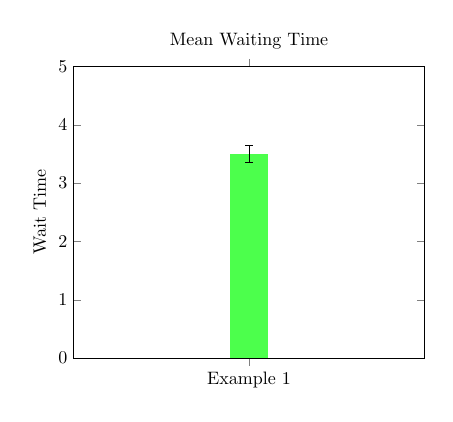
\begin{tikzpicture}[scale=0.65]
\begin{axis}[
ybar, axis on top, title={Mean Waiting Time}, bar width = 0.75cm,
ymin = 0, ymax = 5, ylabel = {Wait Time},
symbolic x coords = {Example 1}, xtick=data
]
\addplot [draw=none, fill=green!70, error bars/.cd, y dir=both, y explicit] coordinates{
	(Example 1, 3.5) -= (0,0.147) += (0,0.147)
};
\end{axis}
\end{tikzpicture}
\end{center}
However, be advised that some graphs use standard deviation for their error bars.
\end{frame}

\begin{frame}{Example 2}
Suppose we take a sample of 45 gas prices and find the mean price per gallon is \$2.45 with a standard deviation of \$0.12. \newline\\
(a)	\quad Create a 98\% confidence interval for the population mean price per gallon.
\begin{align*}
\onslide<2->{& 2.45 \pm 2.326\left(\frac{0.12}{\sqrt{45}}\right)}	\\[8pt]
\onslide<3->{&= 2.45 \pm 0.042} \\[8pt]
\onslide<4->{&= 2.408 \text{ to } 2.492}
\end{align*}
\onslide<5->{A 98\% confidence interval for the mean population price per gallon is \$2.41 to \$2.49}
\end{frame}

\begin{frame}{Example 2}
(b) \quad What would the confidence interval be if the sample size was 100?
\begin{align*}
\onslide<2->{& 2.45 \pm 2.326\left(\frac{0.12}{\sqrt{100}}\right)}	\\[8pt]
\onslide<3->{&= 2.45 \pm 0.012} \\[8pt]
\onslide<4->{&= 2.438 \text{ to } 2.462}
\end{align*}
\onslide<5->{A 98\% confidence interval for the mean population price per gallon is \$2.44 to \$2.46}
\end{frame}

\begin{frame}{Example 2}
(c) \quad Keeping the confidence interval the same, what happens as we increase the sample size?	\newline\\	\pause

Increasing the sample size decreases the standard error. \newline\\	\pause

By doing so, we decrease the width of our confidence interval, while still keeping the confidence level the same. \newline\\	\pause
\end{frame}


\begin{frame}{What the Confidence Interval Is Not}
The following are \alert{incorrect} interpretations of a confidence interval:	\newline\\
\begin{itemize}
	\item<2-> We are \makebox[0.65cm]{\hrulefill}\, \% confident that the population mean is in this interval.	\newline\\
	\item<3-> There is a \makebox[0.65cm]{\hrulefill}\, \% chance that the population mean is (\textit{whatever the sample mean is}).
\end{itemize}
\end{frame}

\section{Determine confidence intervals for population proportion}

\begin{frame}{Mean and Standard Error}
Our point estimate for a population proportion is $\mu_{\hat{p}} = p$ and the standard error is $\sigma_{\hat{p}} = \sqrt{\frac{p(1-p)}{n}}$	\newline\\	\pause

Our confidence interval for the population proportion is
\[p \pm z_{\alpha/2}\sqrt{\frac{p(1-p)}{n}}\]
\end{frame}

\begin{frame}{Example 3}
In a recent sample of 578 voters, 301 of them favored a proposal to renovate a local park. Construct a 90\% confidence interval for the population proportion of voters who favor the renovation.	\newline\\
\onslide<2->{$\hat{p} = \frac{301}{578} \approx 0.521$}
\begin{align*}
\onslide<3->{& 0.521 \pm 1.645 \sqrt{\frac{0.521(0.479)}{578}}}	\\[6pt]
\onslide<4->{&= 0.521 \pm 1.645(0.0208)}	\\[6pt]
\onslide<5->{&= 0.521 \pm 0.034}	\\[6pt]
\onslide<6->{&= (0.487, \, 0.555)}
\end{align*}
\onslide<7->{A 90\% confidence interval for the population proportion of voters who favor the renovation is 48.7 to 55.5\%}
\end{frame}

\begin{frame}{Example 4}
The results of a sample of 40 students who took a pass/fail statistics exam are shown below. Construct a 98\% confidence interval for the population proportion of students who passed the exam.	\newline\\
\begin{tabular}{cccccccc}
Pass & Pass & Fail & Pass & Pass & Pass & Fail & Pass \\
Fail & Pass & Pass & Pass & Fail & Pass & Pass & Pass \\
Pass & Fail & Fail & Pass & Pass & Fail & Pass & Pass \\
Pass & Pass & Fail & Fail & Pass & Pass & Pass & Fail \\
\end{tabular}
\end{frame}

\begin{frame}{Example 4}
\[p = 0.75\]
\begin{align*}
\onslide<2->{& 0.75 \pm 2.326\sqrt{\frac{0.75(0.25)}{40}}}	\\[6pt]
\onslide<3->{&= 0.75 \pm 2.326(0.030)}	\\[6pt]
\onslide<4->{&= 0.75 \pm 0.070}	\\[6pt]
\onslide<5->{&= (0.68, \, 0.82)}
\end{align*}
\onslide<6->{A 98\% confidence interval for the population proportion of students who passed the exam is 68 to 82\%.}
\end{frame}

\section{Determine the necessary sample size}

\begin{frame}{Margin of Error for Population Mean}
Our margin of error, $E$, for a population mean has been given as 
\[E = z_{\alpha/2}\left(\frac{\sigma}{\sqrt{n}}\right)\]
\onslide<2->{Solving for $n$:}
\begin{align*}
\onslide<3->{\frac{E}{z_{\alpha/2}} &= \frac{\sigma}{\sqrt{n}}} \\[6pt]
\onslide<4->{E\sqrt{n} &= \sigma \cdot z_{\alpha/2}} \\[6pt]
\onslide<5->{\sqrt{n} &= \frac{\sigma \cdot z_{\alpha/2}}{E}}	\\[6pt]
\onslide<6->{n &= \left(\frac{\sigma \cdot z_{\alpha/2}}{E}\right)^2}
\end{align*}
\end{frame}

\begin{frame}{Example 5}
How large of a sample size should we take if we want to create a 95\% confidence interval that is within \$0.02 per gallon of the mean cost of gasoline? Assume the standard deviation is \$0.12.
\begin{align*}
\onslide<2->{n &= \left(\frac{\sigma \cdot z_{\alpha/2}}{E}\right)^2}	\\[6pt]
\onslide<3->{n &= \left(\frac{0.12 \cdot 1.96}{0.02}\right)^2}			\\[6pt]
\onslide<4->{n &= 138.2976 \onslide<5->{\rightarrow 139}}
\end{align*}

\onslide<6->{We would need a sample of at least 139.}
\end{frame}

\begin{frame}{Sample Size for Population Proportion}
If we solve	\bigskip
\[E = z_{\alpha/2}\sqrt{\frac{p(1-p)}{n}}\] \bigskip
for $n$, we get	\bigskip
\[n = p(1-p)\left(\frac{z_{\alpha/2}}{E}\right)^2\]

\end{frame}

\begin{frame}{Example 6}
A recent poll shows that 301 out of 578 voters favor renovating a local park. How large of a sample must we take to create a 95\% confidence interval that is within 4\% of the population proportion?	\newline\\	\pause
$p \approx 0.521$
\begin{align*}
\onslide<3->{n &= 0.521(0.479)\left(\frac{1.96}{0.04}\right)^2}	\\[8pt]
\onslide<4->{n &= 599.191159 \onslide<5->{\rightarrow 600}}
\end{align*}

\onslide<5->{We would need a sample size of at least 600.}
\end{frame}

\end{document}